% 第 17 章 Creating Persistent Annotations
\bichapter{创建持久标注}{Creating Persistent Annotations}
\label{chap:gui-anno}

要创建保存在数据库中的持久标注（persistent annotation，包括形状、文本和符号），使用 \cmd{create\_annotation\_shape}、\cmd{create\_annotation\_text} 和 \cmd{create\_annotation\_symbol} 命令。也可以用 Create Annotation 工具（\textbf{Create > Annotation}）来创建。

在 Create Annotation 工具中选中 Attach 复选框后，指针下方的对象会被预先选中。在这样的对象上单击时，标注会附着或锚定到该对象。移动该对象时，标注随之移动。

本章包括以下主题：
\begin{itemize}
  \item 创建标注形状
  \item 创建标注符号
  \item 创建标注文本
  \item 编辑持久标注
  \item 删除持久标注
\end{itemize}

\section{创建标注形状}
\subsection*{Creating Annotation Shapes}

使用 \cmd{create\_annotation\_shape} 命令创建标注形状，类型为圆形（circle）、直线（line）、矩形（rectangle）和多边形（polygon），并可带可选的文本标签。该命令的更多信息见 man 页。

也可以用 Create Annotation 工具创建标注形状。用该工具可以指定类型（circle、rectangle 等）、样式（style，包括填充图案 fill pattern、线宽 line width、颜色等）、标签，以及标签方向（R0、MY 等）。

下列示例用 \cmd{create\_annotation\_shape} 命令创建不同类型的标注形状。
\begin{itemize}
  \item 添加一个绿色矩形标注。
\end{itemize}
\begin{lstlisting}
icc2_shell> create_annotation_shape -type rect -color green \
   -annotation_points {{200 200} {777 777}}
\end{lstlisting}
\begin{itemize}
  \item 添加一条宽度为 2 的红色直线标注。
\end{itemize}
\begin{lstlisting}
icc2_shell> create_annotation_shape -type line \
   -color red -line_width 2 \
   -annotation_points {{123 456} {789 12} {200 200}}
\end{lstlisting}
\begin{itemize}
  \item 添加一个多边形。
\end{itemize}
\begin{lstlisting}
icc2_shell> create_annotation_shape -type polygon \
   -annotation_points {{800 700} {850 700} {900 650} \
   {900 600} {800 600}} -color orange
\end{lstlisting}
\begin{itemize}
  \item 添加一个圆，圆心位于单元 \cmd{I\_CLOCK\_GEN/I\_PLL\_PC} 的中心，半径为 50。
\end{itemize}
\begin{lstlisting}
icc2_shell> create_annotation_shape -type circle \
   -annotation_points [list [get_cells I_CLOCK_GEN/I_PLL_PCI] \
   {50+ 0+}]
\end{lstlisting}

\section{创建标注符号}
\subsection*{Creating Annotation Symbols}

使用 \cmd{create\_annotation\_symbol} 命令创建标注符号，类型包括十字（cross）、菱形（diamond）、正方形（square）、三角形（triangle）、自定义符号，以及随缩放变化的符号（\cmd{fit\_symbol}）。对于自定义符号，必须用 \opt{-file} 选项指定 SVG 格式的输入文件。该命令的更多信息见 man 页。

也可以用 Create Annotation 工具创建标注符号。用该工具可以指定类型（symbol）、具体符号类型、尺寸、样式（填充图案、线宽、颜色等）、符号方向等。

\cmd{fit\_symbol} 类型的标注由预定义形状构成，例如十字、菱形、正方形、三角形或自定义形状。放大时它画得更大，缩小时它画得更小。相比之下，symbol 与文本标注不随缩放变化（zoom-independent），尺寸分别由以像素（pixel）计的符号尺寸和以磅（point）计的字号决定。若符号需要与所标注的物理设计对象保持可比较的尺寸，使用 \cmd{fit\_symbol} 标注。

下列示例用 \cmd{create\_annotation\_symbol} 命令创建不同类型的标注符号。
\begin{itemize}
  \item 添加一个红色菱形标注，填充为十字图案（CrossPattern）。
\end{itemize}
\begin{lstlisting}
icc2_shell> create_annotation_symbol -type diamond \
   -origin {430.490 629.800} -name annoDiamond \
   -size 15 -color red -fill CrossPattern \
   -pen_style SolidLine -pen_width 2
\end{lstlisting}
\begin{itemize}
  \item 添加一个绿色正方形标注，填充为实心图案（SolidPattern）。
\end{itemize}
\begin{lstlisting}
icc2_shell> create_annotation_symbol -type square \
   -origin {534.440 629.800} -name annoSquare \
   -size 15 -color green -fill SolidPattern \
   -pen_style DotLine -pen_width 1
\end{lstlisting}
\begin{itemize}
  \item 添加一个蓝色三角形，中心位于单元 \cmd{I\_CLOCK\_GEN/I\_PLL\_PC} 的中心，并使用图案填充。
\end{itemize}
\begin{lstlisting}
icc2_shell> create_annotation_symbol -type triangle \
   -origin [list [get_cells I_CLOCK_GEN/I_PLL_PCI]] \
   -name annoTriangle -size 75 -color blue -fill Dense7Pattern \
   -pen_style SolidLine -pen_width 1
\end{lstlisting}
\begin{itemize}
  \item 添加一个 \cmd{fit\_symbol} 类型的标注，它随缩放变化。与 \opt{-fit\_symbol} 选项一起使用的必选选项为：\opt{-origin}、\opt{-width} 和 \opt{-height}。
\end{itemize}
\begin{lstlisting}
icc2_shell> create_annotation_symbol -type triangle \
   -origin {430.490 629.800} -fit_symbol -width 200 -height 200
\end{lstlisting}
\begin{itemize}
  \item 用 \opt{-file} 和 \opt{-type} 选项，从 SVG 文件添加标注符号。
\end{itemize}
\begin{lstlisting}
icc2_shell> create_annotation_symbol -type custom \
   -origin {534.440 629.800} -name annoCustom \
   -file star.svg
\end{lstlisting}

要从示例目录添加自定义符号（例如缓冲器 buffer、反相器 inverter、或门 OR gate 或星形 star）：
\begin{enumerate}
  \item （可选）用应用选项（application option）\appopt{gui.annotation\_symbol\_dir} 指定标注符号文件的位置。默认情况下，它指向示例目录。需要时，把该选项改为引用存放 SVG 文件的某个特定目录。
\end{enumerate}
\begin{lstlisting}
icc2_shell> set_app_options -name gui.annotation_symbol_dir \
   -value $synopsys_root/auxx/gui/nwtn/svg_examples
\end{lstlisting}
\begin{enumerate}
  \setcounter{enumi}{1}
  \item 选择 \textbf{Create > Annotation}。
  \item 从 Symbol 下拉列表中选择 custom。
  \item 从 User symbol 下拉列表中选择一个符号。
\end{enumerate}

对于从 SVG 文件添加的符号：
\begin{itemize}
  \item 符号的路径数据（path data）取自 SVG 文件。工具识别 SVG 文件中的下列属性：
  \begin{itemize}
    \item M = moveto（移动到）
    \item L = lineto（直线到）
    \item Q = quadratic Bézier curve（二次贝塞尔曲线）
    \item A = elliptical arc（椭圆弧）
    \item Z = closepath（闭合路径）
  \end{itemize}
  \item 要设置符号的颜色、填充图案等，使用 \cmd{create\_annotation\_symbol} 命令的选项。
\end{itemize}

\section{创建标注文本}
\subsection*{Creating Annotation Text}

使用 \cmd{create\_annotation\_text} 命令创建标注文本。

也可以用 Create Annotation 工具创建标注文本。用该工具可以指定类型（text）、样式（填充图案、线宽、颜色等）、标签、标签方向（R0、MY 等）。Text 栏支持多行文本。

下列示例用 \cmd{create\_annotation\_text} 命令创建不同的标注文本。
\begin{itemize}
  \item 添加水平方向的文本标注。
\end{itemize}
\begin{lstlisting}
icc2_shell> create_annotation_text -text Text1 \
   -origin {969.370 1204.625} -name annoText1 \
   -font_size 12 -color red -horizontal_alignment center \
   -vertical_alignment middle
\end{lstlisting}
\begin{itemize}
  \item 添加垂直方向的文本标注。
\end{itemize}
\begin{lstlisting}
icc2_shell> create_annotation_text -text Text2 \
   -origin {969.370 1204.625} -name annoText2 \
   -font_size 12 -color green -horizontal_alignment center \
   -vertical_alignment middle -orientation vertical
\end{lstlisting}
\begin{itemize}
  \item 添加多行标注文本。
\end{itemize}
\begin{lstlisting}
icc2_shell> create_annotation_text -text "Text3\nText4" \
   -origin {1000.370 1204.625} -name annoText3 \
   -font_size 14 -color red
\end{lstlisting}
\begin{itemize}
  \item 添加相对锚点对象（anchor object）中心有偏移的标注文本。在 GUI 中选中一个对象，并使用下列命令：
\end{itemize}
\begin{lstlisting}
icc2_shell> set object [get_selection]
icc2_shell> create_annotation_text -text "Text5" \
   -origin [list $object bbox_center 25% 25%] -color yellow
\end{lstlisting}

\section{编辑持久标注}
\subsection*{Editing Persistent Annotations}

可以移动、旋转、复制和拉伸已经加到设计中的持久标注。允许的操作见表~\ref{tab:gui-anno-ops}。

\begin{table}[htbp]
\centering
\caption{持久标注允许的操作}
\label{tab:gui-anno-ops}
\footnotesize
\begin{tabularx}{\textwidth}{@{}>{\raggedright\arraybackslash}p{2.7cm}*{7}{>{\centering\arraybackslash}X}@{}}
\toprule
操作 & 圆形 & 直线 & 多边形 & 矩形 & 符号 & fit\_symbol & 文本 \\
\midrule
移动\newline\textbf{Edit > Move}
  & 是 & 是 & 是 & 是 & 是 & 是 & 是 \\
\addlinespace
旋转\newline\textbf{Edit > Move}
  & 否 & 是 & 是 & 是 & 是，并可设方向 & 是，并可设方向 & 是，并可设方向 \\
\addlinespace
复制\newline\textbf{Edit > Copy}
  & 是 & 是 & 是 & 是 & 是 & 是 & 是 \\
\addlinespace
拉伸\newline\textbf{Edit > Stretch}
  & 是 & 是 & 是 & 是 & 是 & 否 & 否 \\
\bottomrule
\end{tabularx}
\end{table}

选中标注后，可以在 Properties Editor 面板中编辑其属性，以调整字号、设置颜色，以及执行其他操作。

\subsection{调整符号尺寸的示例}
\subsubsection*{Example of Resizing Symbols}

在工具中，可以拉伸或调整部分符号标注的尺寸（\textbf{Edit > Stretch}），例如星形、圆形或直线。例如：

\begin{figure}[htbp]
\centering
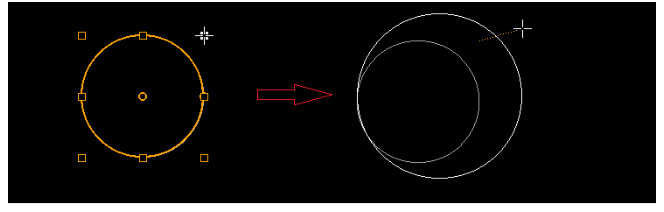
\includegraphics[width=0.92\textwidth]{gui-fig-191.png}
\caption{调整圆形尺寸：拖拽热点（hotspot）以改变尺寸}
\label{fig:gui-191}
\end{figure}

\begin{figure}[htbp]
\centering
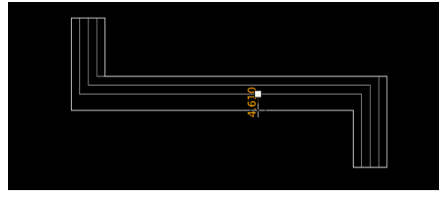
\includegraphics[width=0.92\textwidth]{gui-fig-192.png}
\caption{调整直线：单击并拖拽直线边界以调整线宽}
\label{fig:gui-192}
\end{figure}

\section{删除持久标注}
\subsection*{Removing Persistent Annotations}

要删除某个特定的标注形状：
\begin{enumerate}
  \item 选中该标注形状。
  \item 单击 Delete 工具按钮。
\end{enumerate}

也可以使用 \cmd{remove\_annotation\_shapes [get\_selection]} 命令。

\begin{lstlisting}
icc2_shell> remove_annotation_shapes [get_selection]
\end{lstlisting}
